\section{Analyse paramétrique}
\paragraph{} Après avoir conçu l'outil de gestion du plant, il est intéressant d'analyser les résultats obtenus en
faisant varier les paramètres dans une plage réaliste. Les tableaux ci-dessous reprennent cette analyse. Nous avons
considéré une variation de température de \unit{800}{\kelvin} à \unit{1300}{\kelvin}. Ce choix a été déterminé par
les valeurs de référence utilisées dans le calcul de $K(T)$, qui sont pour la plupart valables jusqu'à
\unit{1300}{\kelvin}. En ce qui concerne la quantité d'ammoniac produite, nous avons testé de \unit{1000}{\ton \per jour} à
\unit{2000}{\ton \per jour}, étant donné que c'est la capacité typique d'un plant d'ammoniac.

\paragraph{} Le premier tableau fait varier la température, en considérant la quantité d'ammoniac \ce{NH_3} produite
par jour constante et valant \unit{1500}{\ton \per jour}.
\begin{table}[h!]
\centering
\begin{tabular}{|c||c|c|c|}
\hline
Température & Débit de méthane \ce{CH_4} & Débit de l'eau \ce{H_{2}O} & Débit d'air \\
\left[$\kelvin$] & [\unit{\meter^3\per jour}] & [\unit{\meter^3\per jour}] & [\unit{\meter^3\per jour}] \\
\hline
800 & 623.30 & 8477.52 & 2258.32 \\
\hline
900 & 623.30 & 3544.50 & 2258.33 \\
\hline
1000 & 623.30 & 1520.12 & 2258.33 \\
\hline
1100 & 623.30 & 626.26 & 2258.33 \\
\hline
1200 & 623.30 & 337.71 & 2258.33 \\
\hline
1300 & 623.30 & 285.73 & 2258.33 \\
\hline
\end{tabular}
\caption{La température $T$ varie, la quantité d'ammoniac \ce{NH_3} produite par jour est constante}
\label{tab:tvarie}
\end{table}

\paragraph{} Le deuxième tableau fait varier la quantité d'ammoniac \ce{NH_3}, en considérant la température $T$ constante et
valant \unit{1000}{\kelvin}.
\begin{table}[h!]
\centering
\begin{tabular}{|c||c|c|c|}
\hline
Production journalière de \ce{NH_3} & Débit de méthane \ce{CH_4} & Débit de l'eau \ce{H_{2}O} & Débit d'air \\
\left[$\ton \per$ jour] & [\unit{\meter^3\per jour}] & [\unit{\meter^3\per jour}] & [\unit{\meter^3\per jour}] \\
\hline
\hline
1000 & 415.53 & 1013.41 & 1505.55 \\
\hline
1200 & 498.64 & 1216.09 & 1806.66 \\
\hline
1400 & 581.74 & 1418.77 & 2107.77 \\
\hline
1600 & 664.85 & 1621.46 & 2408.88 \\
\hline
1800 & 747.96 & 1824.14 & 2709.99 \\
\hline
2000 & 831.06 & 2026.82 & 3011.10 \\
\hline
\end{tabular}
\caption{La quantité d'ammoniac \ce{NH_3} produite par jour varie, la température $T$ est constante}
\label{tab:nh3varie}
\end{table}

\newpage
Nous devions surtout surveiller la quantité d'eau, étant donné qu'elle devait être en excès dans les réactions à
l'équilibre, pour qu'il reste assez de vapeur afin de permettre une conversion complète de \ce{CO} en \ce{CO2} dans le
réacteur Water-Gas-Shift.
Nous avons donc déterminé la température critique à partir de laquelle la quantité d'eau sortante devenait nulle.
Nous sommes arrivés à la conclusion qu'il faut limiter la température de sortie du reformeur primaire à
\unit{1049.472}{\kelvin}, si nous voulons une capacité d'ammoniac de \unit{1500}{\ton\per jour}.
Le graphe suivant permet de visualiser ce qui sort vraiment de notre installation. Les valeurs ont été calculées pour
avoir \unit{1500}{\tonne} d'ammoniac au final. Il est donc normal de constater que l'ammoniac apparaît en ligne droite.
Nous pouvons également bien visualiser qu'à partir de la température de \unit{1050}{\kelvin}, le débit d'eau sortant devient
négatif; chose problématique comme expliqué ci-dessus.
Le \ce{CO2} et l'argon sortant sont quant à eux constants en fonction de la température. L'argon est rejeté en petites quantités mais le \ce{CO2}
apparaît en quantités plus importantes malheureusement.
\begin{figure}[ht!]
\centering
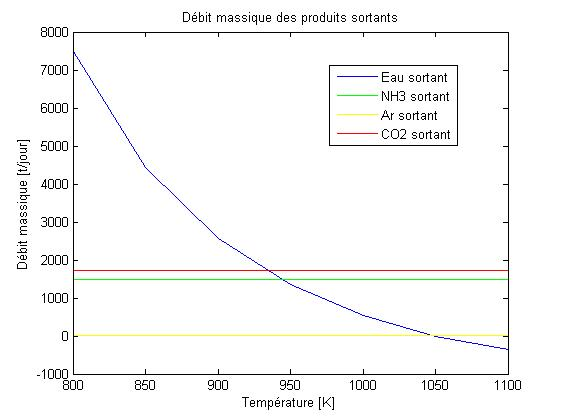
\includegraphics[scale=0.6]{produits.jpg}
\label{produits_sortants}
\end{figure}
